\documentclass{scrartcl}
\usepackage[mathletters]{ucs}
\usepackage[utf8x]{inputenc}
\usepackage{amssymb}
\usepackage{amsmath}
\usepackage[usenames]{color}
\usepackage{hyperref}
\usepackage{wasysym}
\usepackage{graphicx}
\usepackage[normalem]{ulem}
\usepackage{enumerate}

\usepackage{listings}

\lstset{ %
basicstyle=\footnotesize,       % the size of the fonts that are used for the code
showspaces=false,               % show spaces adding particular underscores
showstringspaces=false,         % underline spaces within strings
showtabs=false,                 % show tabs within strings adding particular underscores
frame=single,                   % adds a frame around the code
tabsize=2,                      % sets default tabsize to 2 spaces
breaklines=true,                % sets automatic line breaking
breakatwhitespace=false,        % sets if automatic breaks should only happen at whitespace
}


\title{White Led Strips}
\date{dinsdag 08 december 2020}
\author{}

\begin{document}

\maketitle

		\section{White Led Strips}

Created Wednesday 28 October 2020



A second lighting contition created is the lighting with 3 the same led strips controllable with a raspberry pi. 

This was tested using some transistors to create a controllable switching circuit. This didn't work due to the wrong type of transistors. The second option is to control the led strips using proper relays. These will have to be bought separately so is must still be assessed if this is needed.



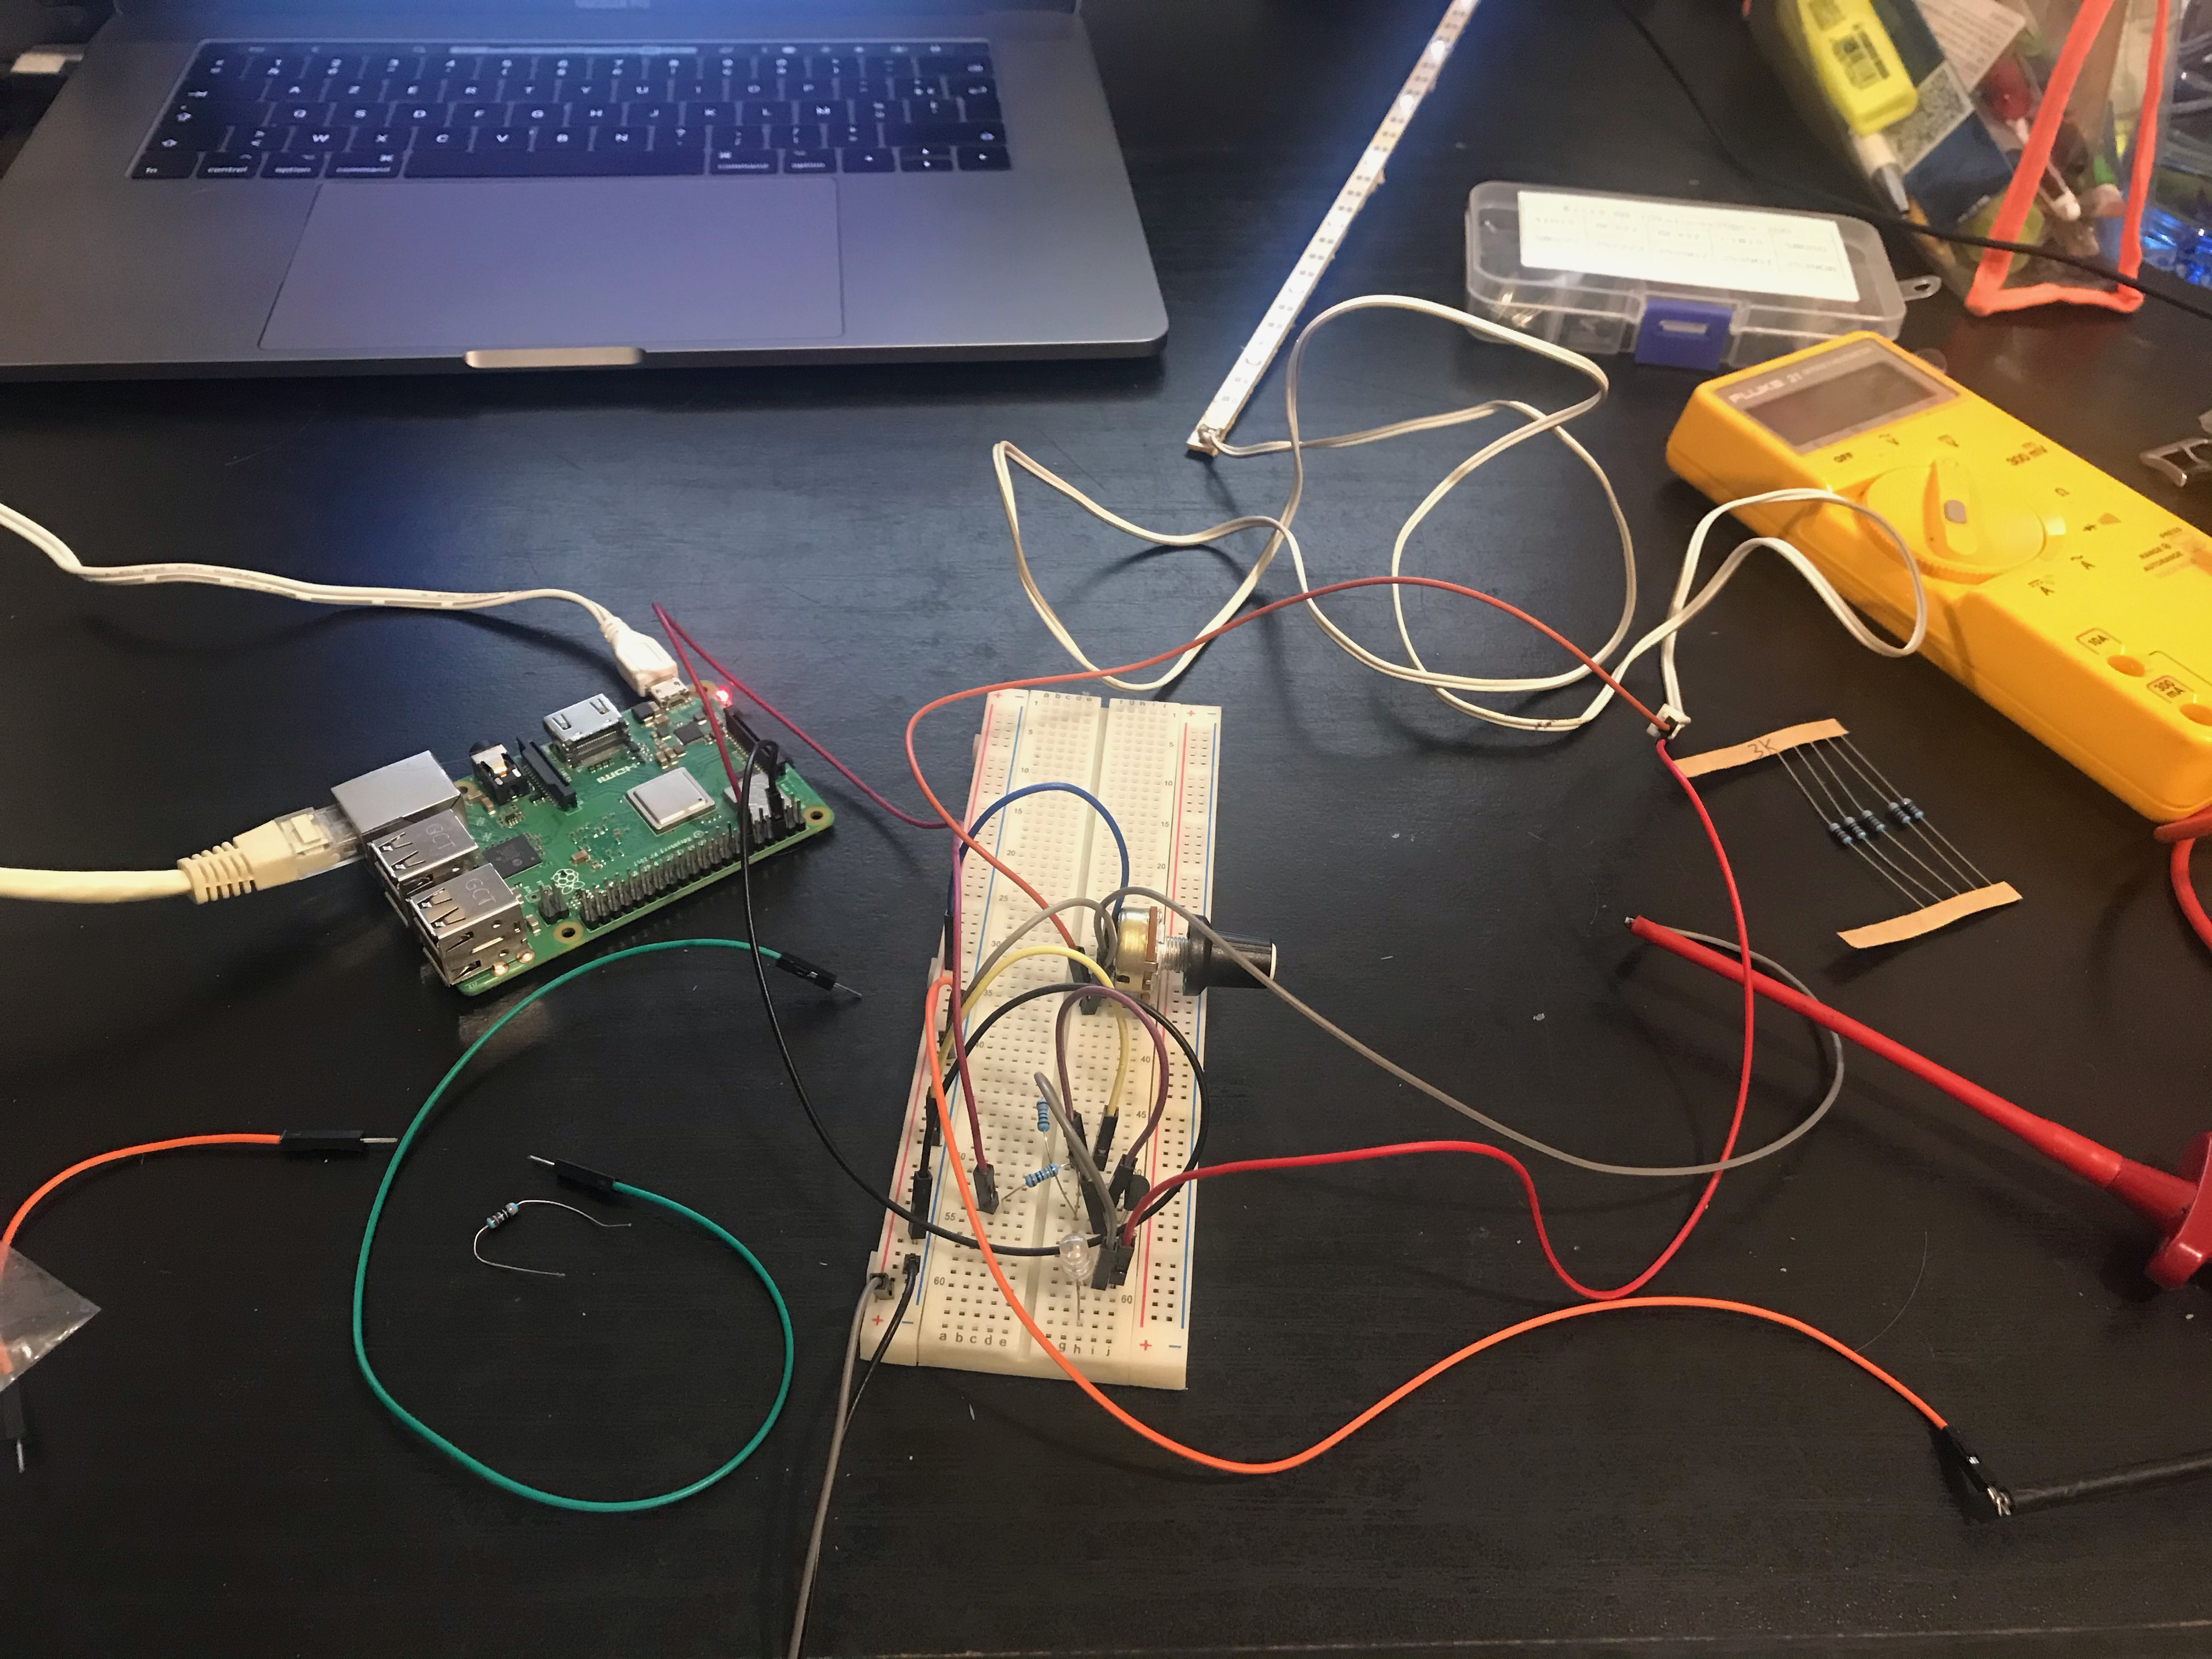
\includegraphics[height=3.125000in, keepaspectratio=true]{./White_Led_Strips/Test_setup_ledstrip.jpeg}

The setup to test the control of a led strip using a NPN transistor as switch.



\end{document}
